\documentclass[../notes.tex]{subfiles}

\pagestyle{main}
\renewcommand{\chaptermark}[1]{\markboth{\chaptername\ \thechapter\ (#1)}{}}
\setcounter{chapter}{7}

\begin{document}




\chapter{Stability Grab Bag}
\section{Midterm 2 Review}
\begin{itemize}
    \item \marginnote{11/14:}Still 3 problems total and 5 points each.
    \begin{itemize}
        \item The problems will be calculations based on the basic concepts.
        \item Figure out the stable and unstable subspaces of some finite systems.
        \item Figure out whether or not a system is stable.
        \item Prove whether or not a function is planar linear
    \end{itemize}
    \item Starting with the classification of planar linear autonomous systems.
    \begin{itemize}
        \item We have $y'=Ay$ where $A$ is a $2\times 2$ real matrix.
        \item As a result of the realness, the eigenvalues behave regularly, i.e., there are only finitely many types of eigenvalues. These are\dots
        \begin{enumerate}
            \item Real, nonzero, same sign. Depending on the sign, we'll either have a source or a sink. The orbits will be a distorted graph of a power function. If asked to investigate the phase portrait, then we need to figure out the stable and unstable subspaces and clearly indicate a basis. If asked to draw, we need to clearly indicate which subspaces are stable and unstable. We also need to clearly indicate the direction of the phase lines. First case: Everything is stable; second case: Everything is unstable. We draw the eigenspaces as well with arrows on the "axes." Figure \ref{fig:planarRealDiaga}-\ref{fig:planarRealDiagb}.
            \item Real, different sign. One stable and one unstable subspace. We need to clearly indicate how the axes are tilted. Figure \ref{fig:planarRealDiagc}.
            \item $A$ is similar to the Jordan block with zero eigenvalues and 1 in the upper right hand corner. Then
            \begin{equation*}
                A\sim
                \begin{pmatrix}
                    0 & 1\\
                    0 & 0\\
                \end{pmatrix}
                \e[tA] =
                \begin{pmatrix}
                    1 & t\\
                    0 & 1\\
                \end{pmatrix}
            \end{equation*}
            \item Purely imaginary eigenvalues. These must appear in a conjugate pair. The phase diagram will be concentric ellipses, and we essentially have the harmonic oscillator equation. If we have to sketch, we must show how the ellipses are tilted.
            \item Complex eigenvalues $\sigma\pm i\beta$. Either we have a spiral source or a spiral sink. It's meaningless to indicate how the spiral tilts here, so don't bother trying. Determining whether they spin clockwise or counterclockwise. If
            \begin{equation*}
                \begin{pmatrix}
                    x\\
                    y\\
                \end{pmatrix}'
                =
                \begin{pmatrix}
                    0 & 1\\
                    -1 & 0\\
                \end{pmatrix}
                \begin{pmatrix}
                    x\\
                    y\\
                \end{pmatrix}
            \end{equation*}
            then our fundamental solution is
            \begin{equation*}
                \begin{pmatrix}
                    x\\
                    y\\
                \end{pmatrix}'
                =
                \begin{pmatrix}
                    \cos t & \sin t\\
                    -\sin t & \cos t\\
                \end{pmatrix}
                \begin{pmatrix}
                    x\\
                    y\\
                \end{pmatrix}
            \end{equation*}
            and we rotate counterclockwise.
            Since $A^2=-\mu^2 I_2$, $\e[tA]=I_2\cos\mu t+\mu^2I_2\sin t$.
            Negative reverses everything.
            Harmonic oscillator goes counterclockwise.
        \end{enumerate}
        \item There is an online website that gives us phase portraits for an equation. We can use this to help develop intuition.
        \item If you have a set of eigenvectors, how do you know how to tilt it?
        \begin{itemize}
            \item Shao goes over examples of eigenvalues and eigenvectors.
        \end{itemize}
        \item This is not something you need to memorize, but something you need to be able to recover.
    \end{itemize}
    \item This is not a course for math majors; thus, there will not be proofs concerning the contraction mapping principle. We will not be asked to show existence, uniqueness, continuous difference, or differentiability with respect to parameters.
    \item We do need to know Gr\"{o}nwall's inequality, however.
    \item Gr\"{o}nwall's inequality: If $\phi:[p,T]\to\R$ and
    \begin{equation*}
        \phi(t) \leq b+a\int_0^t\phi(\tau)\dd\tau
    \end{equation*}
    then
    \begin{equation*}
        \phi(t) \leq b\e[at]
    \end{equation*}
    \begin{itemize}
        \item Usually stated in the integral form, and we usually only need a special case.
        \item We may need to prove this; the proof mimics the derivation of the Duhamel formula.
        \item $a,b\in\R$.
        \item We need to memorize the proof.
        \item We also need to be able to recognize when we can and should use it. Let $\phi(t)=\Phi'(t)\leq b+a\Phi(t)$, $\Phi(0)=0$. Then $\phi(t) \leq b+a\int_0^t\varphi(\tau)\dd\tau$.
        \item Use it when we want to bound a function that satisfies either an integral or a differential quantity.
        \item This is the only proof in the theory of ODE systems we need to memorize.
    \end{itemize}
    \item We need to master the methods to compute perturbation series.
    \begin{itemize}
        \item Suppose our IVP depends on a parameter $\mu$ differentiably.
        \begin{equation*}
            \dv{y}{t}(t;\mu) = f(t;y(t;\mu);\mu), y(t_0)=x(\mu),\mu\approx 0
        \end{equation*}
        \item If the parameter is close to zer, then you should be able to compute the $\mu$-derivative with respect to the parameter.
        \item By Taylor expanding with respect to the parameter, you should be able to recover solutions that are close to the actual.
        \begin{equation*}
            y(t;\mu) = y_0(t)+y_1(t)\mu+y_2(t)\mu^2+O(\mu^3)
        \end{equation*}
        \item We are typically satisfied with approximations to the second order.
        \item We expand our ODE into a Taylor series of $\mu$. The differentiability with respect to parameters theorem (see Lecture 6.2 or Theorem 2.11 in \textcite{bib:Teschl}) tells us that this is legitimate.
        \begin{align*}
            \dv{t}(y_0(t)) &= f(t;y_0(t);0), y_0(t_0)=x(0)\\
            \dv{t}(y_1(t)) &= \pdv{f}{z}(t;y_0(t);0)y_1(t)+\pdv{f}{\mu}(t;y_0(t);0), y_1(t)=\pdv{x}{\mu}(0)
        \end{align*}
        \item Just know the basic Taylor expansions (trig ones and exponential functions; usually we'll stick to polynomials, though).
        \item Use the ansatz $y(t;\mu)=y_0(t)+y_1(t)\mu+y_2(t)\mu^2+O(\mu^3)$.
        \item Substitute $y(t;\mu)$ into $f(t,y(t;\mu);\mu)$. Expand $f(t;y(t;\mu);\mu)$ into a Taylor series of $\mu$. Balance the coefficients of $\mu^0,\mu^1,\mu^2,\dots$.
        \item Then you will get a series of equations that is theoretically solvable. Then a sequence of ODEs for $y_0(t),y_1(t),y_2(t),\dots$.
        \item Your ODEs for $y_1,y_2,\dots$ should not involve $\mu$ (because they are coefficients in the Taylor expansion with respect to $\mu$. Coefficients of a Taylor series shouldn't involve the argument); if it does, there is something going wrong.
        \item As for the initial value, $y_0(t_0)+y_1(t_0)\mu+y_2(t_0)\mu^2+\cdots$. This implies that something equals $x(\mu)$. The Taylor coefficients of $x(\mu)$ at $\mu=0$.
        \item These are the general steps you use to find the perturbative series expansion.
        \item The computations on the exam will not be too heavy.
        \item If you're still unclear on the calculation, look through the HW answer keys.
    \end{itemize}
    \item Conclusion: The Gr\"{o}nwall's inequality is something we need to remember from the theory; the perturbative procedure is something we need to be able to do.
    \item Why do we expand with respect to $\mu$?
    \begin{itemize}
        \item We do it with respect to $\mu$ because our function is a function of $\mu$. Differentiability and smallness imply we can use the Taylor series.
    \end{itemize}
    \item Shao reiterates: Definitely read through the key to HW5!!! All the steps you will need to do are done completely and in detail.
    \item There will be things that are in HW6 (the one due Friday) that will appear on the exam because we have discussed these things in lecture.
    \item The definitions of Lyapunov stability and asymptotic stability. These will appear in the exam. We need to \emph{clearly} remember the definitions.
    \item Consider $y'=f(y)$, $f(x_0)=0$ (an autonomous system with a fixed point; we can transform our system via $(y-x_0)'=f(x_0+(y-x_0))$ to translate our fixed point to zero; implies $y'=f(x_0+y)$, $y=0$ is a fixed point). We should be able to determine the asymptotic stability near $x_0$ by computing the linearization (i.e., the Jacobian $f'(x_0)$) at the fixed point.
    \begin{itemize}
        \item Regarding determining stability near $x_0$, remember the following theorem.
        \item Theorem: If all eigenvalues of $f'(x_0)$ have negative real parts, then $x_0$ is asymptotically stable. If at least one eigenvalue has real part greater than zero, then $x_0$ is not Lyapunov stable.
        \item We should be able to apply the above criterion in practice.
        \item We should also be able to reproduce the proof of the first part of Lyapunov's theorem (related to a question in HW6).
        \item Lyapunov functions: $f(x_0)=0$. Definition:
        \begin{enumerate}
            \item $L(x)$ is $C^1$ near $x_0$, $L(x_0)=0$. $L(x)>0$ for $x$ near $x_0$.
            \item $\nabla L(x)\cdot f(x)\leq 0$ for $x$ near $x_0$ iff $L(\phi_t(x))\leq L(x)$, $t\geq 0$. If $L(\phi_t(x))$ is always strictly decreasing, then it is a strict Lyapunov function.
        \end{enumerate}
        \item Theorem (Lyapunov's theorem): Usually, we can explicitly determine a Lyapunov function:
        \begin{enumerate}
            \item If there is a Lyapunov function near the fixed point, then it is Lyapunov stable. For trajectories starting at nearby points, the trajectory can never excape nearby points.
            \item If there is a strict Lyapunov function, then it is asymptotically stable.
        \end{enumerate}
        \begin{itemize}
            \item We need to be able to apply this theorem in practice; we don't need to know the proof.
        \end{itemize}
    \end{itemize}
    \item Examples of Lyapunov functions: Newton's second law.
    \begin{itemize}
        \item Suppose you have a particle moving within a potential field with potential function $U$, i.e.,
        \begin{equation*}
            mx'' = -U'(x)
        \end{equation*}
        \item Then by a standard process, you can convert it to a planar linear system by introducing the variable $v$ (the velocity), i.e.,
        \begin{equation*}
            \begin{pmatrix}
                x\\
                v\\
            \end{pmatrix}'
            =
            \begin{pmatrix}
                v\\
                -U(x)'/m\\
            \end{pmatrix}
        \end{equation*}
        \item Then $E(x,v)=\frac{m}{2}v^2+U(x)$ is constant along the orbits, that is,
        \begin{equation*}
            \nabla E(x,v)\cdot
            \begin{pmatrix}
                v\\
                -U'(x)/m\\
            \end{pmatrix}
            = 0
        \end{equation*}
        \begin{itemize}
            \item The gradient of the energy function is orthogonal to the vector field.
        \end{itemize}
        \item $E(x,v)$ is a Lyapunov function (global). This happens and induces a fixed point exactly where the velocity is zero and the function takes on a critical value.
        \item Linearization at the fixed point $(x_0,0)$ is
        \begin{equation*}
            \begin{pmatrix}
                0 & 1\\
                -\frac{U''(x_0)}{m} & 0\\
            \end{pmatrix}
        \end{equation*}
        So $E(x_0,v)>E(x_0,0)$ for $x\sim x_0$, $v\sim 0$ iff $U$ takes a minimum at $x_0$. The energy function cannot always stay larger than the energy at the fixed point. Satisfies second Lyapunov condition, but not the first.
        \item One question: Classification of planar linear autonomous systems, one on Gr\"{o}nwall, one on qualitative asymptotic analysis using Lyapunov. Three questions total. There will also be some questions (parts of questions, I guess) on perturbative series.
    \end{itemize}
\end{itemize}



\section{Misc. Stability Tools}
\begin{itemize}
    \item \marginnote{11/18:}Let $y'=f(y)$, where $f:\R^n\to\R^n$ is a smooth function and $x_0$ is a fixed point (i.e., $f(x_0)=0$).
    \item \textbf{Hyperbolic} (fixed point of $f$): A fixed point $x_0\in\R^n$ for which $f'(x_0)$ has neither purely imaginary nor zero eigenvalues.
    \item If $x_0$ is a hyperbolic fixed point of $A$, then we know that for the linear system $y'=Ay$, the eigenvalues of $A$ are never purely imaginary by definition.
    \begin{itemize}
        \item This allows us to decompose $\R^n$ into the direct sum of the \textbf{stable subspace} and the \textbf{unstable subspace} of the system.
    \end{itemize}
    \item \textbf{Stable subspace} (of $x_0$ under $A$): The space of all generalized eigenvectors of $A$ corresponding to eigenvalues $\lambda$ with $\Ree\lambda<0$. \emph{Also known as} \textbf{attracting subspace}. \emph{Denoted by} $\bm{\pmb{\mathbb{E}}_s}$.
    \item \textbf{Unstable subspace} (of $x_0$ under $A$): The space of all generalized eigenvectors of $A$ corresponding to eigenvalues $\lambda$ with $\Ree\lambda>0$. \emph{Also known as} \textbf{repelling subspace}. \emph{Denoted by} $\bm{\pmb{\mathbb{E}}_u}$.
    \item But what if $f$ is not a linear transformation? Then we cannot guarantee the subspace structure, so we need to generalize.
    \item \textbf{Stable subset} (of $x_0$ under $f$): The set of all vectors attracted to $x_0$. \emph{Also known as} \textbf{attracting subset}. \emph{Denoted by} $\bm{W_s(x_0)}$. \emph{Given by}
    \begin{equation*}
        W_s(x_0) = \{x\in\R^n\mid\phi_t(x)\to x_0\text{ as }t\to +\infty\}
    \end{equation*}
    \item \textbf{Unstable subset} (of $x_0$ under $f$): The set of all vectors repelled from $x_0$. \emph{Also known as} \textbf{repelling subset}. \emph{Denoted by} $\bm{W_u(x_0)}$. \emph{Given by}
    \begin{equation*}
        W_u(x_0) = \{x\in\R^n\mid\phi_t(x)\to x_0\text{ as }t\to -\infty\}
    \end{equation*}
    \item Notice that if $f=A$, then the stable (resp. unstable) subset equals the stable (resp. unstable) subspace.
    \item Theorem (stable manifold theorem): Let $y'=f(y)$ and let $x_0$ be a hyperbolic fixed point of $f$. Then there exists a neighborhood $U(x_0)$ of $x_0$ such that $U(x_0)\cap W_s(x_0)$ is a smooth submanifold of dimension $\dim\mathbb{E}_s[f'(x_0)]$ that is tangent to $\mathbb{E}_s[f'(x_0)]$ at $x_0$. An analogous statement holds for $U(x_0)\cap W_u(x_0)$.
    \item \textbf{$\bm{k}$-dimensional smooth submanifold} (of $\R^n$): A subset congruent to the graph
    \begin{equation*}
        G = (w_1,\dots,w_k;h_1(w),\dots,h_{n-k}(w))
    \end{equation*}
    of some smooth function $h:\R^k\to\R^{n-k}$.
    \item Example: $(w,w^2)$ is a 1-dimensional submanifold of $\R^2$.
    \begin{itemize}
        \item We know it as the graph of the unit parabola.
    \end{itemize}
    \item Example: $\left( w_1,w_2,\sqrt{1-(w_1^2+w_2^2)} \right)$ is a 2-dimensional submanifold of $\R^3$.
    \begin{itemize}
        \item In particular, it is the positive hemisphere of the unit two-sphere.
    \end{itemize}
    \item \textbf{Homeomorphism}: A continuous, invertible function with continuous inverse.
    \begin{itemize}
        \item Essentially, it's a coordinate change function.
    \end{itemize}
    \item Theorem (Hartman-Grobman Theorem): Let $y'=f(y)$, $x_0$ a hyperbolic fixed point, and $A=f'(x_0)$. Then there exists a neighborhood $U(x_0)$ and a homeomorphism $h:U(x_0)\to B(x_0,d)$ such that
    \begin{equation*}
        h\circ\phi_t = \e[tA]\circ h
    \end{equation*}
    for $|t|$ small.
    \begin{figure}[h!]
        \centering
        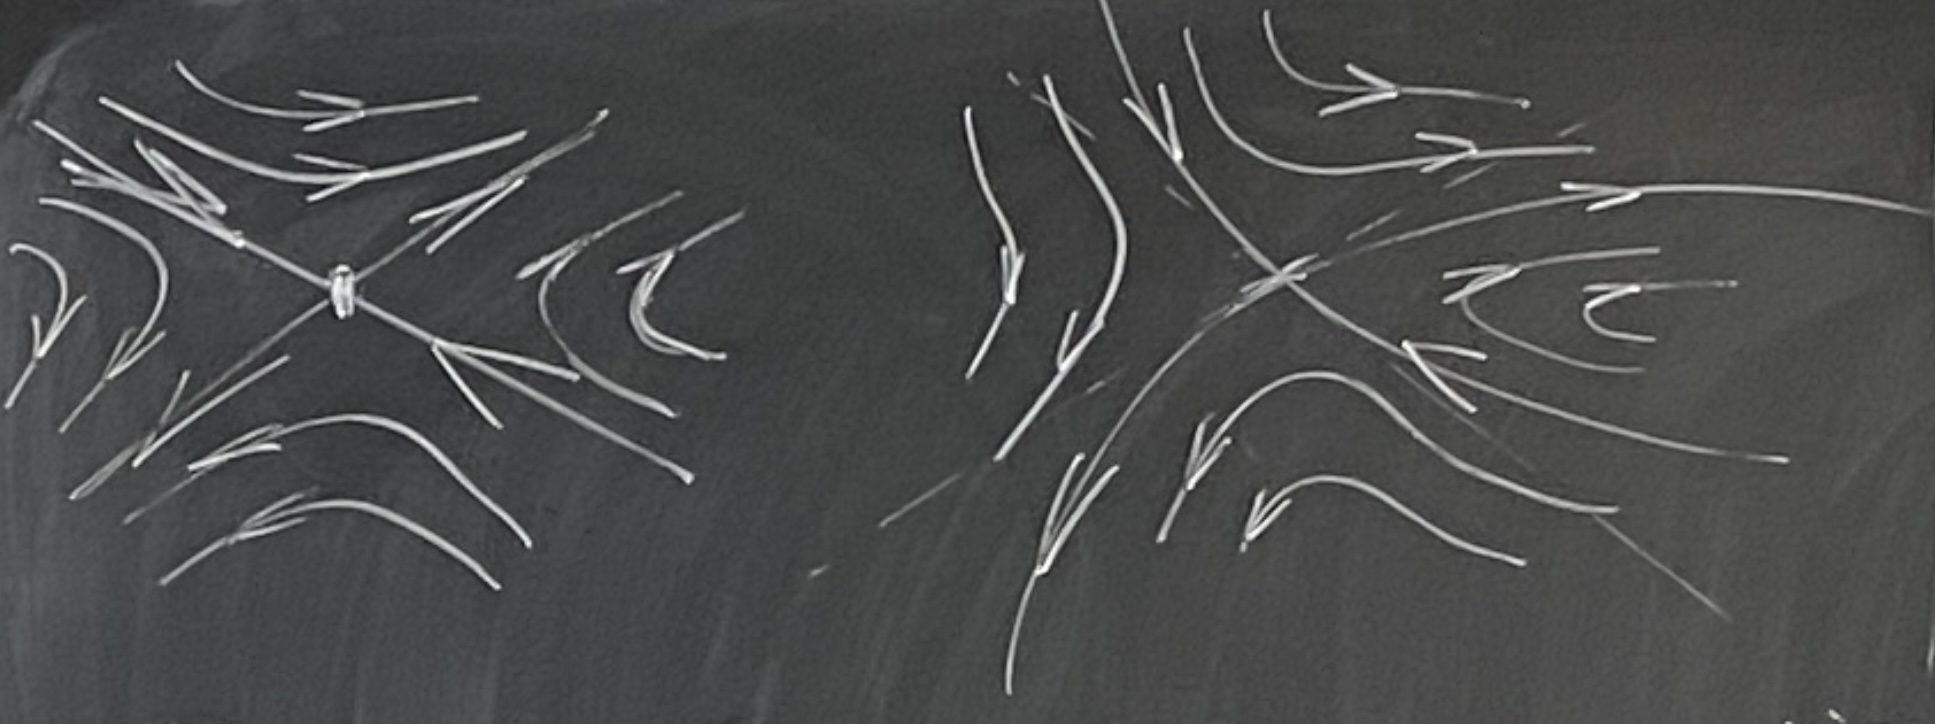
\includegraphics[width=0.6\linewidth]{../ExtFiles/HartmanGrobmanTrm.jpg}
        \caption{Hartman-Grobman Theorem visualization.}
        \label{fig:HartmanGrobmanTrm}
    \end{figure}
    \begin{itemize}
        \item In laymen's terms: Near the hyperbolic fixed point, the orbits are just slight distortions of the linearized system.
    \end{itemize}
    \item Corollary: Suppose $A,B$ are matrices with no purely imaginary eigenvalues. Then the flows of $A,B$ are topologically conjugate iff $\dim\mathbb{E}_s(A)=\dim\mathbb{E}_s(B)$ (equivalently, iff $\dim\mathbb{E}_u(A)=\dim\mathbb{E}_u(B)$).
    \item Example: Let
    \begin{align*}
        A &=
        \begin{pmatrix}
            1 & 1\\
            0 & 1\\
        \end{pmatrix}&
        B &=
        \begin{pmatrix}
            1 & 0\\
            0 & 1\\
        \end{pmatrix}
    \end{align*}
    \begin{figure}[h!]
        \centering
        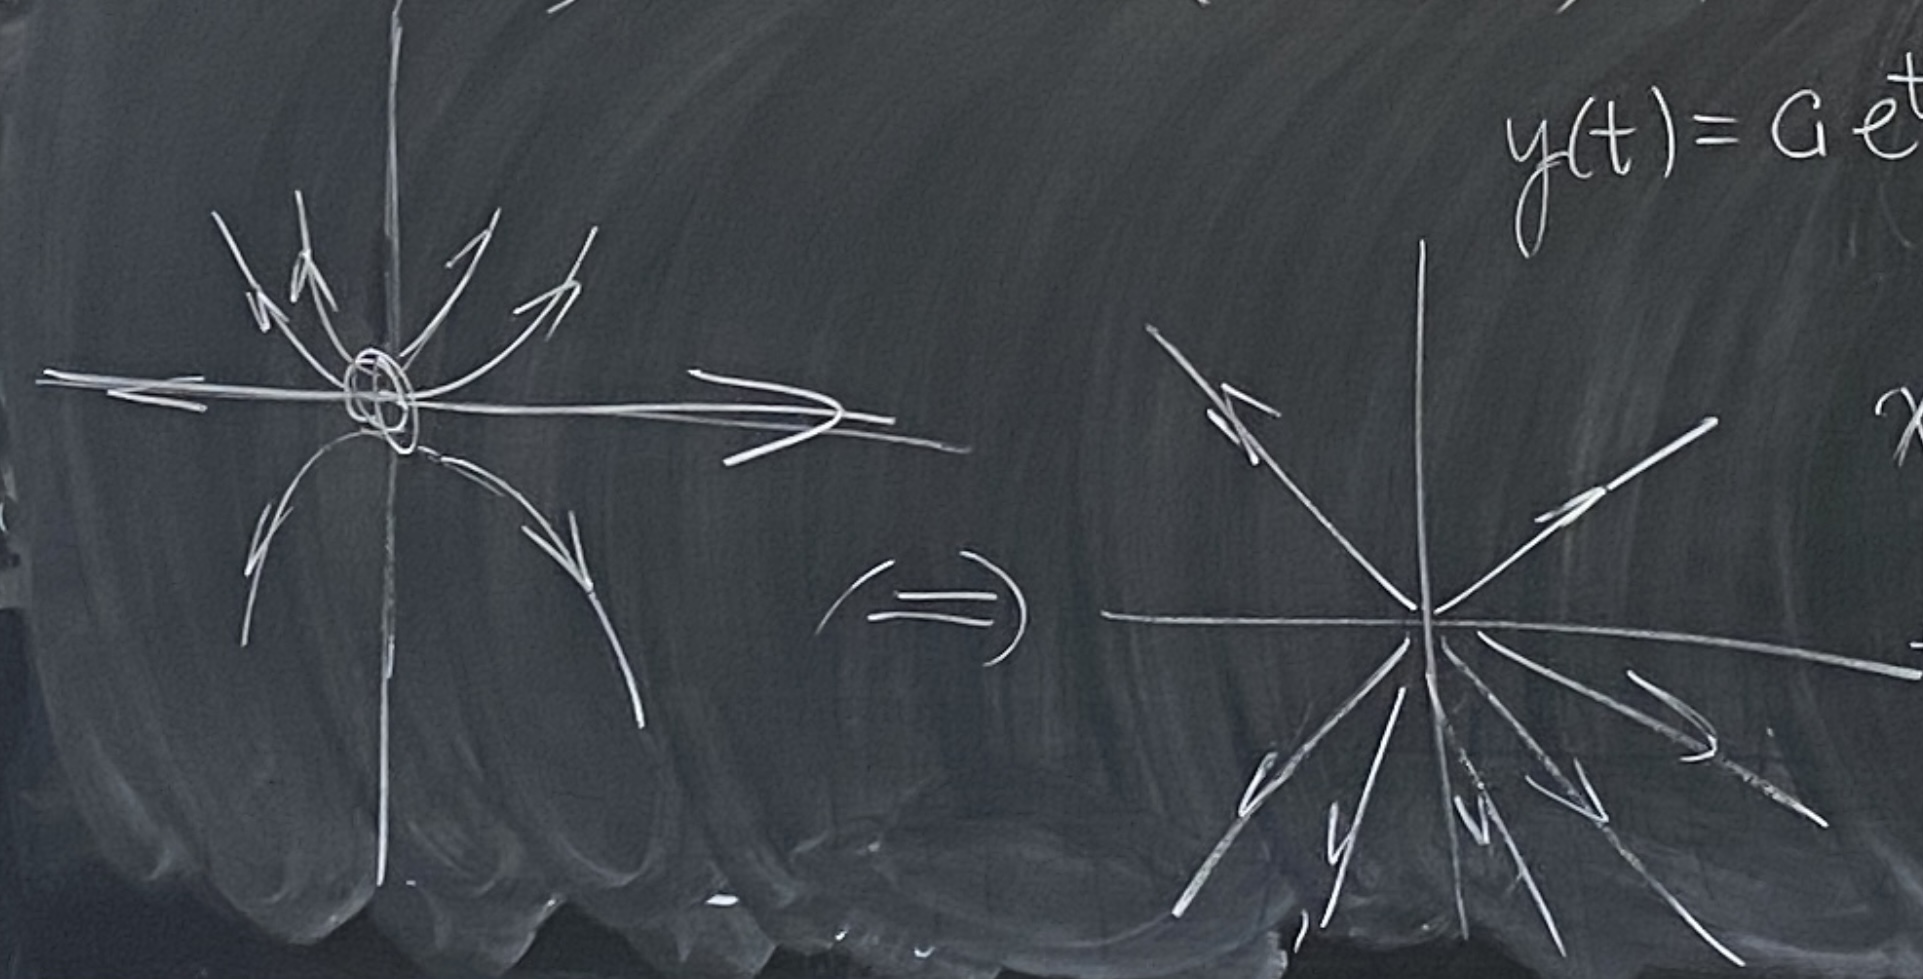
\includegraphics[width=0.6\linewidth]{../ExtFiles/conjFlows.jpg}
        \caption{Topologically conjugate flows.}
        \label{fig:conjFlows}
    \end{figure}
    \begin{itemize}
        \item Consider the linear autonomous systems $y'=Ay$ and $x'=Bx$.
        \item Then since
        \begin{align*}
            \e[tA] &=
            \begin{pmatrix}
                \e[t] & t\e[t]\\
                0 & \e[t]\\
            \end{pmatrix}&
            \e[tB] &=
            \begin{pmatrix}
                \e[t] & 0\\
                0 & \e[t]\\
            \end{pmatrix}
        \end{align*}
        we know that the flows are
        \begin{align*}
            y(t) &=
            \begin{pmatrix}
                \e[t] & t\e[t]\\
                0 & \e[t]\\
            \end{pmatrix}
            \begin{pmatrix}
                c_1\\
                c_2\\
            \end{pmatrix}
                = c_1\e[t]
                \begin{pmatrix}
                    1\\
                    0\\
                \end{pmatrix}
                +c_2\e[t]
                \begin{pmatrix}
                    t\\
                    1\\
                \end{pmatrix}\\
            x(t) &=
            \begin{pmatrix}
                \e[t] & 0\\
                0 & \e[t]\\
            \end{pmatrix}
            \begin{pmatrix}
                c_1\\
                c_2\\
            \end{pmatrix}
                = c_1\e[t]
                \begin{pmatrix}
                    1\\
                    0\\
                \end{pmatrix}
                +c_2\e[t]
                \begin{pmatrix}
                    0\\
                    1\\
                \end{pmatrix}
        \end{align*}
        \item Since both $A,B$ have no purely imaginary eigenvalues, these flows will be topologically conjugate by the Corollary.
        \begin{itemize}
            \item Indeed, we can kind of see that one is a distortion of the other in Figure \ref{fig:conjFlows}.
        \end{itemize}
        \item We can't expect the coordinate change from Hartman-Grobman to be smooth, but it will exist.
    \end{itemize}
    \item Example: Let
    \begin{equation*}
        \begin{pmatrix}
            x\\
            y\\
        \end{pmatrix}'
        =
        \begin{pmatrix}
            -x+y+3y^2\\
            y\\
        \end{pmatrix}
    \end{equation*}
    \begin{itemize}
        \item We can solve this to get
        \begin{equation*}
            \phi_t
            \begin{pmatrix}
                z\\
                w\\
            \end{pmatrix}
            =
            \begin{pmatrix}
                z\e[-t]+w\sinh(t)+w^2(\e[2t]-\e[-t])\\
                w\e[t]\\
            \end{pmatrix}
        \end{equation*}
        \item Notice that the origin 0 is a fixed point.
        \item From this, we can determine that (how??)
        \begin{align*}
            W_s(0) &= x\text{-axis}&
            W_u(0) &= \left\{ \left( \frac{y}{2}+y^2,y \right) \,\middle|\, y\in\R \right\}
        \end{align*}
    \end{itemize}
    \item What if we can't solve the system in the above example explicitly?
    \begin{itemize}
        \item Take the Jacobian at 0:
        \begin{equation*}
            A =
            \begin{pmatrix}
                -1 & 1\\
                0 & 1\\
            \end{pmatrix}
        \end{equation*}
        \item Find its stable and unstable subspaces. Calculate eigenvalues and eigenvectors to be
        \begin{align*}
            \lambda_1 &= -1&
                \lambda_2 &= 1\\
            v_1 &=
            \begin{pmatrix}
                1\\
                0\\
            \end{pmatrix}&
                v_2 &=
                \begin{pmatrix}
                    1\\
                    2\\
                \end{pmatrix}
        \end{align*}
        \item Thus, we get $v_1$ (the $x$-axis) as the stable subspace, and $v_2$ as the unstable subspace.
    \end{itemize}
    \item General procedure for planar systems:
    \begin{enumerate}
        \item Find all fixed points.
        \item Determine the stability of the fixed points. If hyperbolic, then apply the stable manifold and Hartman theorems. If the eigenvalues are purely imaginary, try to find a Lyapunov function.
        \item Decompose the plane into regions in which the monotonicity of
        \begin{equation*}
            \begin{pmatrix}
                x(t)\\
                y(t)\\
            \end{pmatrix}
        \end{equation*}
        is determined, i.e., the signs of the two components of the vector field are determined. This step requires more improvisation.
    \end{enumerate}
    \item Example:
    \begin{equation*}
        \begin{pmatrix}
            \theta\\
            \omega\\
        \end{pmatrix}'
        =
        \begin{pmatrix}
            \omega\\
            -\sin\theta\\
        \end{pmatrix}
    \end{equation*}
    \emph{picture}
    \begin{itemize}
        \item We only care where $-\pi<\theta<\pi$. The fixed points are
        \begin{align*}
            \begin{pmatrix}
                0\\
                0\\
            \end{pmatrix}&&
            \pm
            \begin{pmatrix}
                \pi\\
                0\\
            \end{pmatrix}
        \end{align*}
        \item At 0, the linearization has purely imaginary eigenvalues. We have Lyapunov function
        \begin{equation*}
            E(\theta,\omega) = \frac{1}{2}\omega^2+(1-\cos\theta)
        \end{equation*}
        \item At $(\pi,0)$, the linearization is
        \begin{equation*}
            \begin{pmatrix}
                0 & 1\\
                1 & 0\\
            \end{pmatrix}
        \end{equation*}
        which has eigenvalues and eigenvectors
        \begin{align*}
            \lambda_1 &= 1&
                \lambda_2 &= -1\\
            v_1 &=
            \begin{pmatrix}
                1\\
                1\\
            \end{pmatrix}&
                v_2 &=
                \begin{pmatrix}
                    -1\\
                    1\\
                \end{pmatrix}
        \end{align*}
        \item Thus, we get orbits around 0 in the $\theta,\omega$ plane and two subspaces that converge/diverge to $(\pi,0)$. All of these lines are compatible tangentially.
    \end{itemize}
\end{itemize}



\section{Chapter 9: Local Behavior Near Fixed Points}
\emph{From \textcite{bib:Teschl}}
\subsection*{Section 9.1: Stability of Linear Systems}
\begin{itemize}
    \item \marginnote{12/6:}Goal for the chapter: "Show that a lot of information on the stability of a flow near a fixed point can be read off by linearizing the system around the fixed point" \parencite[253]{bib:Teschl}.
    \item Recall the stability discussion for linear systems
    \begin{equation*}
        \dot{x} = Ax
    \end{equation*}
    from Section 3.2.
    \begin{itemize}
        \item Additionally, our definition from Section 6.5 is invariant under a linear change of coordinates, so we may work in JCF.
        \item Recall that the long-term behavior is determined by the real part of the eigenvalues.
        \item "In general, it depends on the initial condition, and there are two linear manifolds $E^+(\e[A])$ and $E^-(\e[A])$ such that if we start in $E^+(\e[A])$ (resp. $E^-(\e[A])$), then $x(t)\to 0$ as $t\to +\infty$ (resp. $t\to -\infty$)" \parencite[253]{bib:Teschl}.
    \end{itemize}
\end{itemize}


\subsection*{Section 9.2: Stable and Unstable Manifolds}
\begin{itemize}
    \item Goal: Transfer results from the previous section to nonlinear equations.
    \item \textbf{Stable set} (of a fixed point): The set of all points converging to the fixed point $x_0$ for $t\to +\infty$. \emph{Denoted by} $\bm{W^+(x_0)}$. \emph{Given by}
    \begin{equation*}
        W^+(x_0) = \{x\in M\mid\lim_{t\to +\infty}|\Phi(t,x)-x_0|=0\}
    \end{equation*}
    \item \textbf{Unstable set} (of a fixed point): The set of all points converging to the fixed point $x_0$ for $t\to -\infty$. \emph{Denoted by} $\bm{W^-(x_0)}$. \emph{Given by}
    \begin{equation*}
        W^-(x_0) = \{x\in M\mid\lim_{t\to -\infty}|\Phi(t,x)-x_0|=0\}
    \end{equation*}
    \item Both the stable and unstable sets are invariant under the flow.
    \item We know that for small $t$, the solutions are adequately described by the linearization, but what about for large $t$?
    \begin{itemize}
        \item In this section, we generalize the Section 6.5 result for $n=1$ stability and $A=f'(x_0)$ to higher dimensions.
    \end{itemize}
    \item \textbf{Hyperbolic} (fixed point of $f$): A fixed point $x_0$ for which the linearization $f'(x_0)$ has no eigenvalues with zero real part.
    \begin{itemize}
        \item Note that this is equivalent to the definition from class: The "zero real part" condition can be divided into two cases (equal to zero and nonzero but purely imaginary). This definition says no "zero real part;" that definition says not either of the latter two cases.
    \end{itemize}
\end{itemize}




\end{document}